\documentclass[conference]{IEEEtran}
\IEEEoverridecommandlockouts
% The preceding line is only needed to identify funding in the first footnote. If that is unneeded, please comment it out.

% ---------------------------------------------------------
\usepackage{amsmath,amssymb,amsfonts}
% ---------------------------------------------------------
\usepackage{booktabs}
% \usepackage[table,xcdraw]{xcolor}
\usepackage{multirow}
\usepackage{tabularx}
\usepackage{longtable}

% ---------------------------------------------------------
\usepackage{graphicx}
% \usepackage{subcaption}
\usepackage{float}
\usepackage{pdflscape}
\usepackage{lscape}

% ---------------------------------------------------------
\usepackage{algorithm}
\usepackage{algpseudocode}
% ---------------------------------------------------------


% ---------------------------------------------------------
\usepackage{soul}
\usepackage{seqsplit}
\usepackage{url}
% ---------------------------------------------------------
\usepackage{tikz}
\usetikzlibrary{positioning,arrows.meta}

% ---------------------------------------------------------
\usepackage{pgfplots}
\pgfplotsset{compat=1.18}
\usepackage{pgfplotstable}

\usepackage{cite}
\usepackage{textcomp}
\usepackage{xcolor}
% Marker for CLEI 2026 review-response changes. Wrap text to highlight in red.
\newcommand{\new}[1]{{\color{red}#1}}
\def\BibTeX{{\rm B\kern-.05em{\sc i\kern-.025em b}\kern-.08em
    T\kern-.1667em\lower.7ex\hbox{E}\kern-.125emX}}

\begin{document}

\title{Impact of Input Membership Function Design on Fuzzy-Adaptive Particle Swarm Optimization: An Empirical Sensitivity Analysis}
% \thanks{Identify applicable funding agency here. If none, delete this.}


\author{\IEEEauthorblockN{1\textsuperscript{st} José Barrera-García}
\IEEEauthorblockA{\textit{Pontificia Univ. Católica de Valparaíso, Chile} \\
\textit{Universidad de Alcalá, Spain}\\
jose.barrera@pucv.cl}
\and
\IEEEauthorblockN{2\textsuperscript{nd} Broderick Crawford}
\IEEEauthorblockA{\textit{Escuela de Ingeniería Informática} \\
\textit{Pontificia Univ. Católica de Valparaíso}\\
Valparaíso, Chile \\
broderick.crawford@pucv.cl}
\and
\IEEEauthorblockN{3\textsuperscript{rd} José Manuel Gómez-Pulido}
\IEEEauthorblockA{\textit{
Department of Computer Science} \\
\textit{ Universidad de Alcalá}\\
Alcalá de Henares, Spain \\
jose.gomez@uah.es}
\and
\IEEEauthorblockN{4\textsuperscript{th} Felipe Cisternas-Caneo}
\IEEEauthorblockA{\textit{Pontificia Univ. Católica de Valparaíso, Chile} \\
\textit{Universidad de Alcalá, Spain}\\
felipe.cisternas.c@mail.pucv.cl}
\and
\IEEEauthorblockN{5\textsuperscript{th} Ricardo Soto}
\IEEEauthorblockA{\textit{Escuela de Ingeniería Informática} \\
\textit{Pontificia Univ. Católica de Valparaíso}\\
Valparaíso, Chile \\
ricardo.soto@pucv.cl}
\and
\IEEEauthorblockN{6\textsuperscript{th} Eduardo Rodriguez-Tello}
\IEEEauthorblockA{\textit{CINVESTAV} \\
Tamaulipas, Mexico \\
ertello@cinvestav.mx}
\and
\IEEEauthorblockN{7\textsuperscript{th} Yoslandy Lazo}
\IEEEauthorblockA{\textit{Escuela de Ingeniería Informática} \\
\textit{Pontificia Univ. Católica de Valparaíso}\\
Valparaíso, Chile \\
yoslandy.lazo@pucv.cl}
}

\maketitle

\begin{abstract}
This study investigates the impact of input membership function design on the performance of a fuzzy-controlled Particle Swarm Optimization (PSO). Although fuzzy PSO research has typically adopted input partitions without systematic comparison, this work isolates the effect of varying the linguistic representation of iteration progress and population diversity by holding the output set and rule base constant. Four input set geometries crossed with two granularity levels are evaluated on six benchmark functions spanning unimodal and multimodal problem types. Results show a problem-type-dependent pattern: on unimodal functions the baseline PSO with linear inertia weight outperforms all fuzzy variants, whereas on the multimodal problems tested the fuzzy controller improves mean fitness by up to 22.9\% and reduces variability by up to 63\%. Within the fuzzy-controlled variants, the choice of input partition geometry measurably affects performance, with moderate-overlap configurations and three-label granularity yielding the most robust results across the benchmark suite.
\end{abstract}

\begin{IEEEkeywords}
Particle Swarm Optimization, fuzzy logic, inertia weight, membership functions, linguistic granularity, adaptive parameter control
\end{IEEEkeywords}


%%%%%%%%%%%%%%%%%%%%%%%%%%%%%%%%%%%%%%%%%%%%%%%%%%%
%%%%%%%%%%%%%%%%%%%%% SECTION %%%%%%%%%%%%%%%%%%%%%
%%%%%%%%%%%%%%%%%%%%%%%%%%%%%%%%%%%%%%%%%%%%%%%%%%%
\section{Introduction}

Particle Swarm Optimization (PSO) is a population-based metaheuristic whose convergence behavior depends heavily on how global exploration and local exploitation are balanced \cite{kennedy1995particle}. The inertia weight is the main lever for controlling that balance, which has motivated a long line of adaptive strategies \cite{shi1998modified}.

Fuzzy control systems offer a way to adapt PSO parameters online through qualitative descriptions of the search state, and have been used as an alternative to deterministic or iteration-based schedules \cite{shi2001fuzzy}. In practice, however, most fuzzy-controlled PSO variants adopt fixed linguistic partitions and predefined membership functions chosen a priori. How these partitions are shaped is rarely questioned.

Consequently, the effect of linguistic granularity and membership function configuration on PSO performance has not been systematically studied. It remains unclear to what extent different fuzzy linguistic schemes, even under identical control logic, influence optimization behavior across problems with different landscape characteristics.

% [A3 / R1.1] Reformulación de la contribución científica (metodológica/prescriptiva) y scope de generalización.
\new{This paper addresses that gap through a controlled empirical study. Rather than proposing a new algorithm, the contribution is methodological and prescriptive: (i)~it isolates the input membership function partition as an explicit experimental factor, holding the rule base and output set constant so that any performance change is attributable to the input geometry; (ii)~it provides quantitative evidence that this factor is non-negligible, with the choice of partition shape and granularity producing measurable differences in mean fitness and run-to-run variability; and (iii)~it distills a concrete design guideline---moderate-overlap three-label partitions---that researchers and practitioners can adopt as a default starting point when configuring a fuzzy-adaptive PSO.}

\new{The scope of the empirical claims is deliberately bounded by the benchmark suite, which spans both unimodal high-dimensional landscapes (Sphere, Rosenbrock, Griewank in $d{=}100$) and multimodal low-dimensional ones (the Shekel family in $d{=}4$). Within these two regimes the partition-geometry effect is consistent across functions of the same class, which supports a tentative generalization: the qualitative pattern observed---moderate-overlap and coarse-granularity dominate, excessive-overlap and fine-granularity degrade performance---is a property of the controller's interaction with the search state itself, not an artifact of any single benchmark. The findings are therefore most directly applicable to fuzzy-adaptive PSO designs that rely on diversity- and progress-based inputs, which is the dominant pattern in the recent literature~\cite{nobile2018fuzzy, xia2022particle, roy2024hyperparameter, wang2023hierarchical, morales2023stagnation}.}

The rest of the paper proceeds as follows. Section~\ref{sec:related_work} reviews relevant work on fuzzy-adaptive parameter control in PSO and related optimization frameworks. Section~\ref{sec:framework} describes the fuzzy-controlled PSO framework and the linguistic configurations evaluated in this study. Section~\ref{sec:experimental_setup} details the benchmark functions, parameter settings, and experimental protocol. The experimental results and their discussion are presented in Section~\ref{sec:results}. Finally, Section~\ref{sec:conclusions} summarizes the main findings and outlines directions for future research.

%%%%%%%%%%%%%%%%%%%%%%%%%%%%%%%%%%%%%%%%%%%%%%%%%%%
%%%%%%%%%%%%%%%%%%%%% SECTION %%%%%%%%%%%%%%%%%%%%%
%%%%%%%%%%%%%%%%%%%%%%%%%%%%%%%%%%%%%%%%%%%%%%%%%%%
\section{Related Work}
\label{sec:related_work}

Two lines of prior work are relevant here: strategies for adaptive inertia weight control in PSO---particularly those based on fuzzy logic---and studies on how membership function design and linguistic granularity affect fuzzy system behavior.

\subsection{Adaptive Inertia Weight Control in PSO}
\label{subsec:rw_adaptive_w}

Since Shi and Eberhart introduced the inertia weight~\cite{shi1998modified}, many authors have tried to replace the original linear decreasing schedule with state-dependent alternatives. Chatterjee and Siarry~\cite{chatterjee2006nonlinear} introduced nonlinear decreasing functions that accelerate convergence in later iterations, while Nickabadi et al.~\cite{nickabadi2011novel} designed a feedback-based mechanism that adjusts~$w$ according to the swarm's success ratio, coupling the control signal to actual search progress rather than to a predefined temporal schedule.

Fuzzy logic provides a qualitative alternative by encoding adaptation knowledge as linguistic rules. Shi and Eberhart~\cite{shi2001fuzzy} first showed that a Mamdani-type controller driven by swarm performance indicators can outperform static schedules. Their work set the stage for a line of research in which $w$ is governed by linguistic inference rather than by an explicit function of the iteration count. Valdez et al.~\cite{valdez2017comparative} extended this approach with co-evolutionary strategies and showed consistent advantages over classical PSO across diverse benchmarks. Nobile et al.~\cite{nobile2018fuzzy} proposed a self-tuning mechanism that simultaneously adjusts multiple PSO parameters at the particle level, while Xia et al.~\cite{xia2022particle} introduced a multiple-input multiple-output fuzzy controller for adapting learning coefficients and elite selection. Olivas et al.~\cite{olivas2014comparative} showed that interval type-2 controllers can handle additional uncertainty from noisy landscapes, and Roy et al.~\cite{roy2024hyperparameter} recently proposed evolving fuzzy policies that adapt up to seven hyperparameters---arguably the broadest fuzzy control architecture for PSO published so far. % [A5 / R2.1] Referencias 2023--2025 sobre fuzzy-PSO (morales2023, wang2023, li2025rapso).
\new{More recent contributions reinforce the trend toward richer fuzzy adaptation mechanisms: Morales-Casta\~neda et al.~\cite{morales2023stagnation} incorporate a stagnation variable into the fuzzy controller to react to convergence plateaus, Wang et al.~\cite{wang2023hierarchical} introduce a hierarchical fuzzy-logic learning scheme that modulates particle behaviour at multiple levels, and Li et al.~\cite{li2025rapso} combine reinforcement learning with an adaptive weight strategy that conceptually overlaps with fuzzy-driven adaptation.}

A common trait in the works reviewed above is that the input membership functions---defining how diversity, fitness progress, or other indicators are fuzzified---are chosen a priori, and their geometric configuration is seldom examined as an experimental factor. Research efforts have concentrated on rule base design, output set selection, or the number of controlled parameters, while the input partition tends to be treated as a fixed design element.

\subsection{Membership Function Design and Linguistic Granularity}
\label{subsec:rw_mf_design}

Work in the broader fuzzy systems community already points in this direction. Olivas et al.~\cite{olivas2014comparative} demonstrated that different membership function shapes produce statistically significant performance differences even when the rule base remains unchanged, which implies that membership functions carry semantic content beyond their mathematical form. Metaheuristic-based tuning of membership function parameters reinforces this point, having shown sensitivity across several application domains~\cite{fierro2013optimization, nikolic2020bee}.

At the partition level, Cord\'on et al.~\cite{cordon2000uniform} established guidelines for obtaining uniform fuzzy partitions with adequate granularity, showing that properties such as overlap degree and label spacing are constrained by consistency requirements. Guillaume and Charnomordic~\cite{guillaume2004interpretable} proposed methods for generating interpretable partitions from data while preserving semantic coherence. Taken together, these works show that the geometric configuration of membership functions---support width, overlap, and boundary treatment---has a direct effect on both interpretability and control behavior.

A second design axis is the number of linguistic labels used to partition the input space, commonly called linguistic granularity. Castiello et al.~\cite{castiello2019interpretable} showed that adaptive granularity can improve discrimination in classification tasks without sacrificing interpretability. In the context of optimization, Huang et al.~\cite{huang2022linguistic} and Zhang et al.~\cite{zhang2022linguistic} showed that the granularity of linguistic scales affects convergence behavior and solution quality in PSO-related decision-making problems.

Despite this evidence, the specific influence of input membership function geometry and linguistic granularity on fuzzy-controlled PSO has received little dedicated attention. Most fuzzy PSO studies in the literature adopt a single partition---typically three uniformly spaced triangular labels---without comparing it against alternatives. The present work contributes to filling this gap through a factorial design in which four input set geometries, differing in overlap degree and boundary treatment, are crossed with two granularity levels (3 and 5~labels) under a constant output set and rule base. Because everything else is held fixed, differences in performance can be attributed to the input partition itself.
%%%%%%%%%%%%%%%%%%%%%%%%%%%%%%%%%%%%%%%%%%%%%%%%%%%
%%%%%%%%%%%%%%%%%%%%% SECTION %%%%%%%%%%%%%%%%%%%%%
%%%%%%%%%%%%%%%%%%%%%%%%%%%%%%%%%%%%%%%%%%%%%%%%%%%
\section{Fuzzy-Controlled PSO Framework}
\label{sec:framework}

This section describes the PSO framework and the fuzzy control layer added to it. A swarm-level fuzzy inference system adapts the inertia weight at every iteration. The question under study is whether---and how much---the geometric configuration of the \emph{input} membership functions affects the resulting optimization behavior. To answer it, the output fuzzy set and rule base are kept the same across all variants; only the input partition changes.

\subsection{Baseline Particle Swarm Optimization}
\label{subsec:baseline_pso}

A swarm of $N$~particles cooperates to minimise an objective function $f\colon\mathbb{R}^d\to\mathbb{R}$ over a bounded search space $\prod_{k=1}^{d}[L_k, U_k]$, where $d$~denotes the problem dimensionality and $L_k$, $U_k$ are the lower and upper bounds of dimension~$k$. The baseline corresponds to the canonical PSO formulation~\cite{kennedy1995particle, shi1998modified}, where each particle $i$ is characterised by a position $x_i(t)\in\mathbb{R}^d$ and a velocity $v_i(t)\in\mathbb{R}^d$; motion is governed by inertia, cognitive attraction toward the personal best, and social attraction toward the global best position. Particle dynamics are defined by
\begin{equation}
    v_i(t{+}1) = w \cdot v_i(t) + c_1 r_1 \bigl(p_i - x_i(t)\bigr) + c_2 r_2 \bigl(g - x_i(t)\bigr),
    \label{eq:pso_velocity}
\end{equation}
\begin{equation}
    x_i(t{+}1) = x_i(t) + v_i(t{+}1),
    \label{eq:pso_position}
\end{equation}
where $w$ is the inertia weight, $c_1$ and $c_2$ are the cognitive and social acceleration coefficients, $p_i$ and $g$ denote the personal and global best positions, and $r_1, r_2 \in [0,1]$ are uniformly distributed random variables.

In the baseline configuration, the inertia weight follows a deterministic linear decreasing schedule from $0.9$ to $0.1$ over the optimization horizon~\cite{abualigah2021arithmetic}. The acceleration coefficients are set to $c_1 = c_2 = 2.0$ for all configurations. This baseline is the reference against which fuzzy-controlled inertia adaptation is measured.

\subsection{Fuzzy Control System for Inertia Weight Adaptation}
\label{subsec:fcs}

In the fuzzy-controlled variants, a Mamdani-type fuzzy inference system (FIS) is embedded into the PSO loop and evaluated once per iteration at the swarm level. At iteration~$t$, the controller outputs an inertia weight~$w_t$ based on two normalized indicators: iteration progress and population diversity.

Iteration progress is defined as
\begin{equation}
    t_{\text{progress}} = \frac{t}{T_{\max}},
    \label{eq:iteration_progress}
\end{equation}
where $T_{\max}$ is the maximum number of iterations. Population diversity measures the normalized spatial dispersion of the swarm:
\begin{equation}
    D(t) = \frac{1}{d} \sum_{k=1}^{d}
    \frac{\max_i x_{i,k}(t) - \min_i x_{i,k}(t)}{U_k - L_k},
    \label{eq:diversity_metric}
\end{equation}
where $d$ is the problem dimensionality and $[L_k, U_k]$ are the bounds of dimension~$k$.

The fuzzy controller maps these inputs to an inertia weight constrained to $[w_{\min}, w_{\max}]$. Defuzzification is performed using the centroid method:
\begin{equation}
    w_t = \frac{\int_{Z} z \, \mu_{\text{agg}}(z)\, dz}{\int_{Z} \mu_{\text{agg}}(z)\, dz},
    \label{eq:defuzzification}
\end{equation}
% [A2 / R2.2] Descripción completa de los elementos de Ec.~\ref{eq:defuzzification}: z, Z, mu_agg y mapeo afín al rango operativo.
\new{where $z \in Z = [0, 1]$ is the output variable spanning the normalized inertia-weight domain, and $\mu_{\text{agg}}(z) \in [0, 1]$ is the aggregated output membership function obtained by combining (via the max operator) the clipped consequents of all rules activated at iteration~$t$. The resulting $w_t \in [0,1]$ is then affinely mapped to the operational range $[w_{\min}, w_{\max}]$.} Fig.~\ref{fig:fcs_architecture_vertical} illustrates the integration of the fuzzy controller within the PSO iteration loop.


\begin{figure}[ht]
    \centering
    \resizebox{0.75\columnwidth}{!}{
        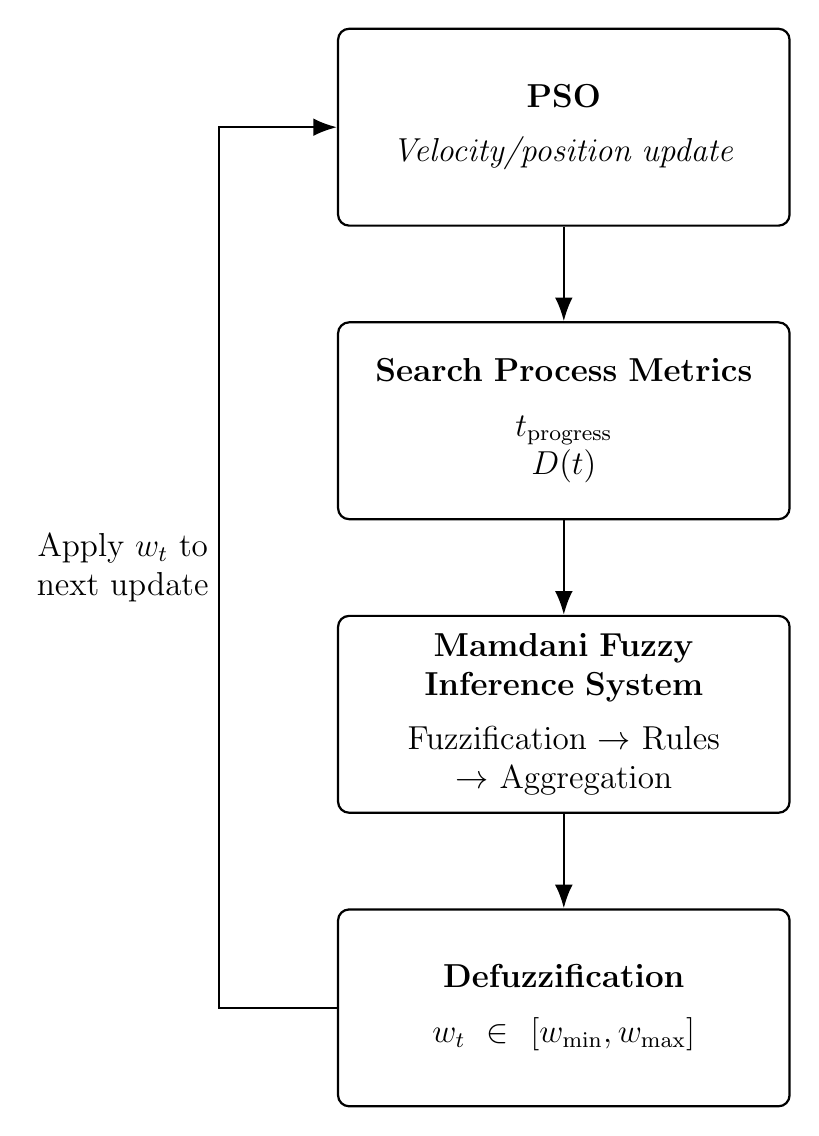
\begin{tikzpicture}[
            font=\large,
            block/.style={
                draw,
                rounded corners,
                align=center,
                minimum height=25mm,
                text width=55mm,
                thick
            },
            arrow/.style={-{Latex[length=3mm]}, thick},
            node distance=12mm
        ]
        
        % Definición de nodos en el eje vertical
        \node[block] (pso) {
            \textbf{PSO}\\
            \vspace{2mm}
            \emph{Velocity/position update}
        };
        
        \node[block, below=of pso] (metrics) {
            \textbf{Search Process Metrics}\\
            \vspace{2mm}
            $t_{\text{progress}}$ \\
            $D(t)$
        };
        
        \node[block, below=of metrics] (fis) {
            \textbf{Mamdani Fuzzy}\\
            \textbf{Inference System}\\
            \vspace{2mm}
            Fuzzification $\rightarrow$ Rules \\
            $\rightarrow$ Aggregation
        };
        
        \node[block, below=of fis] (wt) {
            \textbf{Defuzzification}\\
            \vspace{2mm}
            $w_t \in [w_{\min}, w_{\max}]$
        };
        % Main flow (descending)
        \draw[arrow] (pso) -- (metrics);
        \draw[arrow] (metrics) -- (fis);
        \draw[arrow] (fis) -- (wt);
        
        % Feedback loop
        \draw[arrow] (wt.west) -- ++(-15mm,0) |- 
            node[pos=0.25, left, align=center] {Apply $w_t$ to\\next update} 
            (pso.west);
        
        \end{tikzpicture}
    }
    \caption{Architecture of the Fuzzy-Controlled PSO Framework}
    \label{fig:fcs_architecture_vertical}
\end{figure}

% [B3 / R2.3] Pseudocódigo del FCS-PSO para reproducibilidad (preferido sobre figura de arquitectura).
\new{Algorithm~\ref{alg:fcs_pso} summarizes the resulting procedure. The fuzzy controller is queried once per iteration at the swarm level, so the entire FIS evaluation block is independent of both the population size~$N$ and the problem dimensionality~$d$.}

{\color{red}
\begin{algorithm}[ht]
\caption{Fuzzy-Controlled PSO (FCS--PSO)}
\label{alg:fcs_pso}
\small
\begin{algorithmic}[1]
\Require $f\colon\mathbb{R}^d\to\mathbb{R}$, $T_{\max}$, $N$, $d$, $[L_k,U_k]_{k=1}^{d}$, $[w_{\min}, w_{\max}]$, FIS
\Ensure global best position $g$
\State Initialize $x_i \sim \mathcal{U}([L_k,U_k]_{k=1}^d)$, $v_i \gets \mathbf{0}$ for $i = 1, \dots, N$
\State Evaluate $f(x_i)$; set $p_i \gets x_i$; $g \gets \arg\min_i f(p_i)$
\For{$t = 1$ \textbf{to} $T_{\max}$}
    \State $t_{\text{progress}} \gets t / T_{\max}$ \Comment{Eq.~\eqref{eq:iteration_progress}}
    \State $D(t) \gets \text{diversity}(\{x_i\})$ \Comment{Eq.~\eqref{eq:diversity_metric}}
    \State $w_t \gets \textsc{FIS}.\text{infer}(D(t),\, t_{\text{progress}})$ \Comment{Eq.~\eqref{eq:defuzzification}}
    \For{$i = 1$ \textbf{to} $N$}
        \State Update $v_i$ with $w_t$ \Comment{Eq.~\eqref{eq:pso_velocity}}
        \State Update $x_i$ \Comment{Eq.~\eqref{eq:pso_position}}
        \State Evaluate $f(x_i)$
        \If{$f(x_i) < f(p_i)$} $p_i \gets x_i$ \EndIf
    \EndFor
    \State $g \gets \arg\min_i f(p_i)$
\EndFor
\State \Return $g$
\end{algorithmic}
\end{algorithm}
}

\subsection{Input Membership Function Configurations}
\label{subsec:input_mf_configs}

The central factor under study is the geometric configuration of the input membership functions---the partitions applied to diversity ratio and iteration progress. While prior work on fuzzy-controlled PSO has explored diverse rule bases, multi-parameter tuning, and alternative controller architectures~\cite{shi2001fuzzy, nobile2018fuzzy, xia2022particle}, the sensitivity of the controller to input partition geometry has received limited attention. This work addresses that gap by evaluating four input set configurations, each employing triangular membership functions with different overlap and boundary characteristics.

All four configurations share the same linguistic labels---low, medium, and high for diversity; early, mid, and late for iteration progress---and are applied identically to both input variables. Any difference in controller behavior therefore comes from the shape of the partitions, not from a change in the underlying semantic structure.

\begin{itemize}
    \item \textbf{I1 (Standard):} Uniformly distributed triangular functions with moderate overlap. This is the textbook partition and serves as the default reference.
    \item \textbf{I2 (Narrow):} Reduced support width and zero overlap between adjacent labels. Transitions between linguistic regions are sharper, so the controller switches rules more abruptly.
    \item \textbf{I3 (Wide):} Increased support width with substantial overlap between neighbors. The result is a smoother, more gradual inertia adaptation.
    \item \textbf{I4 (Shoulder):} Shoulder functions at the extremes and a standard triangle at the center. Near domain boundaries the extreme label stays fully active ($\mu = 1$), which locks a single rule in place at extreme input values.
\end{itemize}

Two levels of linguistic granularity are also considered: a three-label partition (low, medium, high) and a five-label one (very\_low, low, medium, high, very\_high). In the five-label case, each input set extends its geometric principles---overlap degree, boundary treatment---to five uniformly spaced labels. Crossing four input geometries with two granularity levels yields eight fuzzy-controlled PSO variants.

Table~\ref{tab:input_sets_3L} details the triangular parameters $(a, b, c)$ for each configuration at both granularity levels. The same partition is applied symmetrically to both input variables.

% [A6 / R1.0] Tablas de parámetros MF 3L y 5L fusionadas en una sola table* con dos bloques.
\begin{table*}[htbp]
    \caption{\new{Triangular membership function parameters $(a, b, c)$ for each input set, at three- and five-label granularity. In I4, extreme labels use shoulder functions where $a{=}b$ or $b{=}c$. I2 achieves zero overlap between adjacent labels at both granularities. The same partition is applied symmetrically to diversity and iteration progress.}}
    \label{tab:input_sets_3L}
    \centering
    \footnotesize
    \setlength{\tabcolsep}{4pt}
    \begin{tabular}{lcccc}
    \toprule
    Label & I1 (Standard) & I2 (Narrow) & I3 (Wide) & I4 (Shoulder) \\
    \midrule
    \multicolumn{5}{l}{\emph{Three-label granularity (9 rules)}}\\
    Low/Early   & $(0.0, 0.2, 0.4)$ & $(0.0, 0.16, 0.33)$ & $(0.0, 0.25, 0.5)$ & $(0.0, 0.0, 0.35)$ \\
    Medium/Mid  & $(0.3, 0.5, 0.7)$ & $(0.33, 0.5, 0.66)$ & $(0.25, 0.5, 0.75)$ & $(0.2, 0.5, 0.8)$ \\
    High/Late   & $(0.6, 0.8, 1.0)$ & $(0.66, 0.84, 1.0)$ & $(0.5, 0.75, 1.0)$ & $(0.65, 1.0, 1.0)$ \\
    \midrule
    \multicolumn{5}{l}{\emph{Five-label granularity (25 rules)}}\\
    Very Low/Very Early & $(0.0, 0.15, 0.3)$  & $(0.0, 0.1, 0.2)$  & $(0.0, 0.15, 0.35)$  & $(0.0, 0.0, 0.25)$  \\
    Low/Early           & $(0.2, 0.35, 0.5)$  & $(0.2, 0.3, 0.4)$  & $(0.15, 0.3, 0.5)$ & $(0.15, 0.3, 0.45)$ \\
    Medium/Mid          & $(0.35, 0.5, 0.65)$ & $(0.4, 0.5, 0.6)$  & $(0.3, 0.5, 0.7)$  & $(0.35, 0.5, 0.65)$ \\
    High/Late           & $(0.5, 0.65, 0.8)$  & $(0.6, 0.7, 0.8)$  & $(0.5, 0.7, 0.85)$  & $(0.55, 0.7, 0.85)$ \\
    Very High/Very Late & $(0.7, 0.85, 1.0)$  & $(0.8, 0.9, 1.0)$  & $(0.65, 0.85, 1.0)$ & $(0.75, 1.0, 1.0)$  \\
    \bottomrule
    \end{tabular}
\end{table*}

\subsection{Output Fuzzy Set Configuration}
\label{subsec:output_set}

The output variable is the inertia weight~$w$, defined over $[0, 1]$ and then scaled to $[w_{\min}, w_{\max}]$. A single output set (Set~A) is shared by all variants so that the output side does not confound the comparison of input partitions.

Set~A employs uniformly distributed triangular membership functions with symmetric overlap. For the three-label case, the output labels are low~$(0.00, 0.25, 0.5)$, medium~$(0.25, 0.50, 0.75)$, and high~$(0.50, 0.75, 1.0)$. The five-label extension subdivides the same domain into very\_low, low, medium, high, and very\_high with equal spacing.

\subsection{Fuzzy Rule Base}
\label{subsec:rule_base}

The rule base encodes how iteration progress and diversity map to inertia weight. The general idea is a standard one: high inertia early in the search or when the swarm has collapsed (low diversity), and low inertia later when the population still covers the space adequately.

The same rule semantics are preserved across all input set configurations and both granularity levels. Tables~\ref{tab:rules3} and~\ref{tab:rules5} present the complete rule bases.

\begin{table}[htbp]
\caption{Fuzzy rule base for inertia weight adaptation (3~labels, 9~rules).}
\label{tab:rules3}
\centering
\begin{tabular}{@{}cccc@{}}
\toprule
Rule & Progress & Diversity & Output $w$ \\ \midrule
1    & early    & low       & high   \\
2    & early    & medium    & high   \\
3    & early    & high      & high   \\\midrule
4    & mid      & low       & low    \\
5    & mid      & medium    & medium \\
6    & mid      & high      & high   \\\midrule
7    & late     & low       & low    \\
8    & late     & medium    & low    \\
9    & late     & high      & medium \\ \bottomrule
\end{tabular}
\end{table}

\begin{table}[htbp]
\caption{Fuzzy rule base for inertia weight adaptation (5~labels, 25~rules).}
\label{tab:rules5}
\centering
\begin{tabular}{@{}cccc@{}}
\toprule
Rule & Progress   & Diversity & Output $w$ \\ \midrule
1  & very early & very low  & very high \\
2  & very early & low       & very high \\
3  & very early & medium    & high      \\
4  & very early & high      & high      \\
5  & very early & very high & medium    \\ \midrule
6  & early      & very low  & very high \\
7  & early      & low       & high      \\
8  & early      & medium    & high      \\
9  & early      & high      & medium    \\
10 & early      & very high & medium    \\ \midrule
11 & mid        & very low  & high      \\
12 & mid        & low       & high      \\
13 & mid        & medium    & medium    \\
14 & mid        & high      & medium    \\
15 & mid        & very high & low       \\ \midrule
16 & late       & very low  & high      \\
17 & late       & low       & medium    \\
18 & late       & medium    & low       \\
19 & late       & high      & low       \\
20 & late       & very high & very low  \\ \midrule
21 & very late  & very low  & medium    \\
22 & very late  & low       & low       \\
23 & very late  & medium    & very low  \\
24 & very late  & high      & very low  \\
25 & very late  & very high & very low  \\ \bottomrule
\end{tabular}
\end{table}



%%%%%%%%%%%%%%%%%%%%%%%%%%%%%%%%%%%%%%%%%%%%%%%%%%%
%%%%%%%%%%%%%%%%%%%%% SECTION %%%%%%%%%%%%%%%%%%%%%
%%%%%%%%%%%%%%%%%%%%%%%%%%%%%%%%%%%%%%%%%%%%%%%%%%%
\section{Experimental Setup}
\label{sec:experimental_setup}

\subsection{Benchmark Functions}
\label{subsec:benchmarks}

The experimental evaluation uses six classical benchmark functions representing two structurally distinct groups: high-dimensional problems with regular landscapes and low-dimensional problems with rugged, deceptive landscapes.

The first group includes three functions evaluated in $d = 100$ dimensions. The Sphere function~(F1) is a unimodal baseline with a smooth, convex landscape. Rosenbrock's function~(F5) provides a unimodal challenge characterized by a narrow, curved valley where convergence is highly sensitive to search direction. Griewank's function~(F11) introduces regular multimodality through oscillatory components superimposed on a quadratic base.

The second group comprises three variants of the Shekel function in a four-dimensional space ($d = 4$), differing in the number of components~$m$: F21~($m{=}5$), F22~($m{=}7$), and F23~($m{=}10$). The Shekel family is characterized by closely spaced deep optima, making it particularly challenging for population-based methods prone to premature convergence.

All functions were evaluated through the \texttt{Opfunu} library~\cite{Van_Thieu_2024_Opfunu}, which provides reference implementations of classical benchmarks. Table~\ref{tab:benchmark_functions} summarizes the selected benchmarks.

\begin{table}[!ht]
    \caption{Benchmark functions used in the experimental evaluation.}
    \label{tab:benchmark_functions}
    \centering
    \begin{tabular}{lcccc}
    \toprule
    Function & Type & Dim. & Bounds & Global Opt. \\
    \midrule
    F1 (Sphere)            & Unimodal   & $100$ & $[-100, 100]^d$ & $0.0$ \\
    F5 (Rosenbrock)        & Unimodal   & $100$ & $[-30, 30]^d$   & $0.0$ \\
    F11 (Griewank)         & Multimodal & $100$ & $[-600, 600]^d$ & $0.0$ \\
    F21 (Shekel, $m{=}5$)  & Multimodal & $4$   & $[0, 10]^d$     & $-10.1532$ \\
    F22 (Shekel, $m{=}7$)  & Multimodal & $4$   & $[0, 10]^d$     & $-10.4029$ \\
    F23 (Shekel, $m{=}10$) & Multimodal & $4$   & $[0, 10]^d$     & $-10.5363$ \\
    \bottomrule
    \end{tabular}
\end{table}

\subsection{Parameter Settings and Evaluation Protocol}
\label{subsec:protocol}

All algorithmic variants were evaluated under identical conditions. The population size was fixed at $50$~particles and the maximum number of iterations was set to $500$. No additional stopping criteria were applied.

Each algorithm--function combination was executed over $31$ independent runs. A shared seeding strategy was adopted: all algorithms used the same random seed for the $k$-th run, with the initial seed set to $42$ and incremented by one for each subsequent run, yielding seeds $\{42, 43, \ldots, 72\}$.

The baseline PSO with linearly decreasing inertia weight was evaluated alongside eight fuzzy-controlled variants (PSO--FCS). These variants result from the full factorial combination of the four input set configurations described in Section~\ref{subsec:input_mf_configs} (I1--I4) and two granularity levels (3 and 5~labels), with the output fuzzy set~(A) and rule base held constant. Table~\ref{tab:algorithm_configs} summarizes the nine configurations, totaling $9 \times 6 \times 31 = 1{,}674$ independent experiments.

\begin{table}[!ht]
    \caption{Algorithm configurations evaluated. All PSO--FCS variants share the same rule base and output set; only input membership functions and granularity vary.}
    \label{tab:algorithm_configs}
    \centering
    \begin{tabular}{lcccc}
    \toprule
    Algorithm & $w$ Control & Output Set & Labels & Input Set \\
    \midrule
    PSO (baseline)   & Linear decrease & --- & --- & --- \\
    PSO--FCS--I1--3L & Fuzzy (FCS) & A & 3 & I1 (Standard) \\
    PSO--FCS--I2--3L & Fuzzy (FCS) & A & 3 & I2 (Narrow) \\
    PSO--FCS--I3--3L & Fuzzy (FCS) & A & 3 & I3 (Wide) \\
    PSO--FCS--I4--3L & Fuzzy (FCS) & A & 3 & I4 (Shoulder) \\
    PSO--FCS--I1--5L & Fuzzy (FCS) & A & 5 & I1 (Standard) \\
    PSO--FCS--I2--5L & Fuzzy (FCS) & A & 5 & I2 (Narrow) \\
    PSO--FCS--I3--5L & Fuzzy (FCS) & A & 5 & I3 (Wide) \\
    PSO--FCS--I4--5L & Fuzzy (FCS) & A & 5 & I4 (Shoulder) \\
    \bottomrule
    \end{tabular}
\end{table}

Performance was assessed using the final best fitness value and the relative gap to the known global optimum, defined as
\begin{equation}
    \text{Gap}(\%) =
    \frac{\left| f_{\text{best}} - f_{\text{opt}} \right|}
    {\left| f_{\text{opt}} \right|} \times 100.
    \label{eq:gap_metric}
\end{equation}
For functions with $f_{\text{opt}} = 0$ (F1, F5, F11), performance is reported directly as the absolute best fitness value, since the relative gap is undefined.

Robustness was evaluated via the mean and standard deviation of final fitness values across the 31~runs. % [A1 / R2.6] Justificación del Wilcoxon signed-rank por estrategia de seeding pareada + rank-sum como complemento.
\new{Statistical significance was assessed primarily with the Wilcoxon signed-rank test at $\alpha = 0.05$. The choice of a paired test is deliberate: the shared seeding strategy ensures that, for any fixed run index~$k$, all algorithms start from the same initial population, so each $k$-th observation of one algorithm is naturally paired with the $k$-th observation of another. Under this design the signed-rank test removes initialization-induced variance and yields higher statistical power than its independent-samples counterpart, in line with established practice in nonparametric comparison of metaheuristics~\cite{derrac2011practical}. The Wilcoxon rank-sum (Mann--Whitney~$U$) test, which treats the two samples as independent, is also reported as a complementary indicator of distributional difference.} Computational cost was measured using wall-clock execution time.

All experiments were conducted on a 64-bit system with an Intel Core~i7 CPU (2.8~GHz) and 16~GB of RAM. The algorithms were implemented in Python~3.11.9 and executed sequentially.




%%%%%%%%%%%%%%%%%%%%%%%%%%%%%%%%%%%%%%%%%%%%%%%%%%%
%%%%%%%%%%%%%%%%%%%%% SECTION %%%%%%%%%%%%%%%%%%%%%
%%%%%%%%%%%%%%%%%%%%%%%%%%%%%%%%%%%%%%%%%%%%%%%%%%%
\section{Results and Discussion}
\label{sec:results}

The results fall into three parts and are discussed below: the overall comparison between baseline PSO and the fuzzy-controlled variants, the effect of input set geometry, and the role of linguistic granularity.

\subsection{Overall Performance: PSO vs PSO--FCS}
\label{subsec:overall_results}

Table~\ref{tab:pso_vs_fcs} summarizes the comparison between the baseline PSO and the best-performing PSO--FCS variant for each benchmark function. All six functions are minimization problems: F1, F5, and F11 have a global optimum of zero, while the Shekel functions F21--F23 have negative global optima ($-10.1532$, $-10.4029$, and $-10.5363$, respectively). The best fuzzy configuration per function was therefore selected by lowest mean fitness across 31~runs in all cases.


% [A1 / R2.6] Tabla actualizada con ambos p-values: signed-rank (p_sr) y rank-sum (p_rs).
\begin{table}[ht]
    \caption{\new{PSO vs best PSO--FCS variant per function. Fitness improvement, standard deviation reduction, Wilcoxon signed-rank ($p_{\text{sr}}$) and rank-sum ($p_{\text{rs}}$) $p$-values, and computational overhead are reported over 31 independent runs.}}
    \label{tab:pso_vs_fcs}
    \centering
    \footnotesize
    \setlength{\tabcolsep}{3pt}
    \begin{tabular}{@{}lclrrrrr@{}}
    \toprule
    Func. & Win & Best FCS & Impr.\% & $\sigma$\,Red.\% & $p_{\text{sr}}$ & $p_{\text{rs}}$ & OH\% \\
    \midrule
    F1  & PSO & I1:3L & --- & --- & $<$0.001\rlap{***} & $<$0.001\rlap{***} & 20.1 \\
    F5  & PSO & I1:5L & --- & --- & $<$0.001\rlap{***} & $<$0.001\rlap{***} & 27.6 \\
    F11 & PSO & I1:3L & --- & --- & $<$0.001\rlap{***} & $<$0.001\rlap{***} & 20.2 \\
    F21 & FCS & I2:5L & $+$22.9 & $-$63.0 & 0.041\rlap{*}     & 0.955\,ns         & 3.6 \\
    F22 & FCS & I1:3L & $+$6.5  & $-$58.7 & 0.824\,ns         & 0.034\rlap{*}     & 5.3 \\
    F23 & FCS & I2:3L & $+$9.9  & $-$57.3 & 0.504\,ns         & 0.127\,ns         & 1.0 \\
    \bottomrule
    \end{tabular}
\end{table}

The results differ markedly between unimodal and multimodal landscapes. On F1, F5, and F11 the baseline PSO achieves fitness values that are orders of magnitude better than any fuzzy variant ($p < 0.001$, Wilcoxon signed-rank test), with 20--28\% less computation time. On unimodal landscapes, the single basin of attraction makes diversity-driven inertia adaptation unnecessary. The fuzzy controller reads the natural convergence of the swarm as low diversity and raises~$w$ to promote exploration---counterproductive when the swarm is already heading toward the global optimum.

On the Shekel functions (F21--F23), the situation is reversed. The best PSO--FCS variant improves mean fitness by 6.5--22.9\% over the baseline and reduces standard deviation by 57--63\%, with negligible overhead (1.0--5.3\%). Here, the fuzzy controller detects premature convergence toward local optima and raises inertia to re-diversify the swarm. The 57--63\% drop in standard deviation across 31~runs indicates that the controller not only improves average quality but also makes the search considerably more repeatable.

% [A7 / R1.4] Discusión de escalabilidad del overhead: el costo del FIS es O(1) por iteración e independiente de d.
\new{The relative overhead of the fuzzy layer is a function of the per-iteration fitness cost, not of the problem dimensionality. The controller performs a fixed amount of work each iteration---two fuzzifications, a small lookup of at most 9~(or 25)~rules, and one centroid defuzzification---all of which are independent of~$d$. The high relative overhead on F1, F5 and F11 (20--28\%) reflects how cheap their fitness evaluations are, not a scaling problem of the FIS itself. On more computationally demanding problems---higher-dimensional landscapes, simulation-based fitness, or surrogate-assisted settings---the same fixed per-iteration cost is amortized over much larger evaluation budgets, so the overhead is expected to become negligible. This is consistent with the 1--5\% values observed on the Shekel functions, whose fitness is itself heavier than the unimodal ones.}

% [A4 / R1.5] Discusión honesta de la no-significancia parcial en F22/F23; los dos tests se interpretan complementariamente.
\new{Statistical significance on the multimodal group is partial and the two tests highlight different aspects of the data. The paired signed-rank test detects a significant per-run advantage of the fuzzy controller on F21 ($p_{\text{sr}} = 0.041$) but not on F22 or F23, while the rank-sum test---which ignores the pairing---finds a significant distributional difference on F22 ($p_{\text{rs}} = 0.034$) and none on F21 or F23. The disagreement is informative rather than contradictory: the Shekel family has closely spaced deep optima, so small changes in initial positions can redirect the swarm to a different attractor, inflating within-sample variance. When the paired structure is preserved (signed-rank), this variance is partially absorbed and a consistent per-seed improvement emerges on F21; when the samples are treated as independent (rank-sum), the broader distributional shift on F22 becomes detectable. In all three multimodal cases the fuzzy controller improves the mean and roughly halves the standard deviation, but these gains should be read as practically meaningful rather than uniformly significant in the strict statistical sense.}

% [B2 / R2.4] Curvas de convergencia (fitness vs iter) para F21--F23: comportamiento online del controlador.
\new{Fig.~\ref{fig:convergence_multimodal} reports the online behaviour of both algorithms on the multimodal benchmarks. Baseline PSO collapses toward its asymptotic mean within roughly 50~iterations but its wide standard-deviation band reveals a bimodal outcome: some runs reach the global optimum while others remain trapped near shallow local optima. The fuzzy controller descends more gradually yet converges to a lower mean with a markedly narrower band, which is the same pattern reported in Table~\ref{tab:pso_vs_fcs}: comparable best-case performance, substantially more consistent average behaviour across seeds.}

{\color{red}
\begin{figure*}[!htbp]
    \centering
    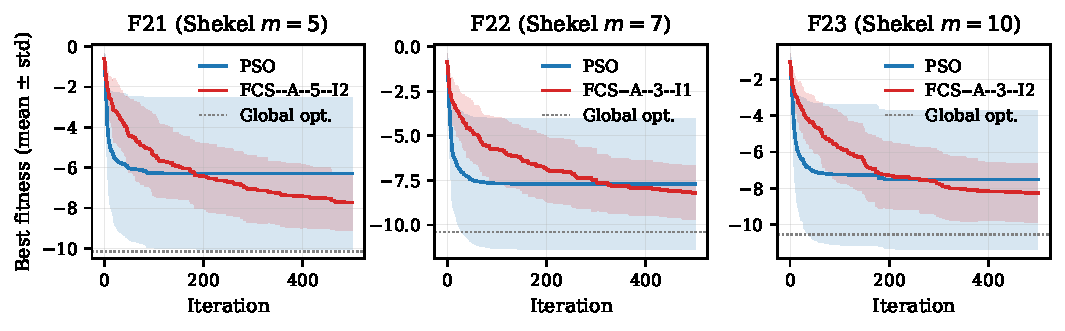
\includegraphics[width=0.85\linewidth]{figures/b2_convergence_multimodal.pdf}
    \caption{Convergence trajectories of the best fitness across 31 independent runs for the multimodal Shekel benchmarks. Solid lines show the mean over runs and shaded bands the $\pm 1$ standard deviation envelope. The dotted line marks the global optimum.}
    \label{fig:convergence_multimodal}
\end{figure*}
}

Fig.~\ref{fig:pso_vs_fcs_boxplot} shows the fitness distributions for all six functions. On the Shekel group, fuzzy variants produce tighter interquartile ranges and fewer extreme outliers than the baseline, while on unimodal functions the gap in favor of standard PSO is visually evident.

\begin{figure*}[!htbp]
    \centering
    \includegraphics[width=\linewidth]{figures/08_pso_vs_fcs_boxplot.png}
    \caption{Fitness distributions (31~runs) for PSO and the best PSO--FCS variant per function. On unimodal functions (F1, F5, F11), PSO dominates. On multimodal functions (F21--F23), the fuzzy-controlled variant achieves better medians and reduced dispersion.}
    \label{fig:pso_vs_fcs_boxplot}
\end{figure*}

Fig.~\ref{fig:scatter_fitness_std} plots mean fitness against standard deviation for all nine configurations on each function, adding a second perspective on the same data. On the Shekel functions the PSO baseline (star marker) sits in the high-variance region, while the FCS variants group toward lower standard deviations. On unimodal functions the picture is the opposite: every FCS configuration lands far from the PSO baseline, well into the worse-fitness region.

\begin{figure*}[p]
    \centering
    \includegraphics[width=0.95\linewidth]{figures/04_scatter_fitness_std.png}
    \caption{Mean fitness vs.\ standard deviation for all configurations on each benchmark function. Colors encode input sets (I1--I4), markers distinguish granularity ($\circ$\,=\,3L, $\square$\,=\,5L), and the star denotes the PSO baseline. On multimodal functions, FCS variants achieve lower dispersion; on unimodal functions, all FCS variants are orders of magnitude worse than PSO.}
    \label{fig:scatter_fitness_std}
\end{figure*}

\subsection{Effect of Input Set Geometry}
\label{subsec:input_geometry}

% [B1-aux] Tabla tab:input_ranking eliminada; los ranks se mueven inline para liberar espacio para la Fig. de activación de reglas (B1).
\new{To determine whether input partition geometry actually matters, the mean rank of each input set across the six benchmark functions was computed separately per granularity level (rank~1 = best on a function; lower average~rank = more consistent performance across the suite). At three labels, I1~(Standard) attains the best average rank at~2.83, followed by I2~(Narrow) at~3.67, I4~(Shoulder) at~4.50, and I3~(Wide) at~5.50. At five labels the ordering is similar (I4~4.00, I1~4.50, I2~5.17, I3~5.83), with I3 again worst. I2's sharper boundaries help on the Shekel functions where the controller must react quickly to diversity drops, while Section~\ref{subsec:granularity} traces the poor performance of I3 to its rule activation pattern.}

Fig.~\ref{fig:heatmap_multimodal} presents the fitness heatmap for the multimodal functions, where the effect of input set geometry is most pronounced. I1 and I2 consistently achieve the darkest (best) cells, while I3 and I4 show lighter (worse) values, particularly on F21 and F22.

\begin{figure*}[p]
    \centering
    \includegraphics[width=0.95\linewidth]{figures/01b_heatmap_multimodal.png}
    \caption{Mean fitness heatmap for multimodal functions (F21--F23) across input sets and granularity levels. Darker cells indicate better fitness. I1 and I2 configurations consistently outperform I3 and I4.}
    \label{fig:heatmap_multimodal}
\end{figure*}

% [B1 / R1.7] Diagnóstico de activación de reglas (exp H) que explica por qué 3L > 5L y por qué I3 (Wide) rinde peor.
\subsection{Effect of Linguistic Granularity \new{and Rule Activation Diagnostics}}
\label{subsec:granularity}

Across the board, three-label partitions outrank their five-label counterparts. Three labels yield a better mean rank for three of the four input sets (I1, I2, I3); only I4~(Shoulder) benefits marginally from the finer partition. The average Gap\% mirrors the trend at 23.7\% versus 24.1\%---a small but consistent margin pointing to over-segmentation when five labels are used.

\new{To probe the mechanism, the recorded $(D(t), t_{\text{progress}})$ trajectories of every run were replayed through each FIS configuration and the effective number of simultaneously active rules per sample was computed as $\exp(H)$, where $H$ is the Shannon entropy of the normalised rule-firing distribution. Shannon entropy was chosen because it is parameter-free---unlike threshold-based rule counts, which require an arbitrary cut-off---and it weights each rule proportionally to its firing strength, so a rule with $\mu{=}0.01$ contributes far less than one with $\mu{=}0.5$. The exponential form maps the result to a natural scale: $\exp(H){=}1$ when exactly one rule fires, and larger values indicate increasingly diffuse firing. Fig.~\ref{fig:rule_activation} aggregates this diagnostic over the $93{,}186$ swarm-level samples per configuration and mirrors the performance ranking. I3~(Wide) attains the highest blending (1.40 at 3L, 1.83 at 5L), confirming that excessive overlap dilutes the control signal across competing rules. I2~(Narrow) sits exactly at~1.0 because its zero-overlap partition admits only one active rule per sample. I1~(Standard) lies in between (1.13 / 1.54), striking the balance that yields its leading mean rank. Moving from 3L to 5L raises the active-rule count for I1 and I3 by 31--36\%, evidence that the additional labels do not introduce finer-grained decisions but rather spread the firing mass over more rules without changing what the controller perceives.}

{\color{red}
\begin{figure}[!htbp]
    \centering
    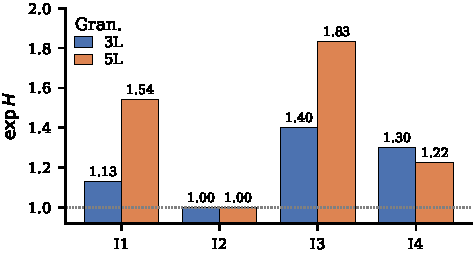
\includegraphics[width=0.95\columnwidth]{figures/b1_rule_activation.pdf}
    \caption{Effective number of simultaneously active rules ($\exp H$) per input set and granularity, over $93{,}186$ recorded $(D(t), t_{\text{progress}})$ samples per configuration. Higher values indicate a more blurred control signal.}
    \label{fig:rule_activation}
\end{figure}
}

% \newpage
%%%%%%%%%%%%%%%%%%%%%%%%%%%%%%%%%%%%%%%%%%%%%%%%%%%
%%%%%%%%%%%%%%%%%%%%% SECTION %%%%%%%%%%%%%%%%%%%%%
%%%%%%%%%%%%%%%%%%%%%%%%%%%%%%%%%%%%%%%%%%%%%%%%%%%
\section{Conclusions}
\label{sec:conclusions}

This work investigated the sensitivity of fuzzy-controlled PSO to the geometric design of input membership functions, a factor that has received limited explicit attention in the literature. By crossing four input set geometries (I1--I4) with two granularity levels (3 and 5~labels) under a constant output set and rule base, a total of 1,674 experiments were conducted across six benchmark functions with distinct landscape characteristics.

The experiments yield three observations.

First, changing the input membership functions does change controller performance by a non-negligible margin. On the Shekel functions the best fuzzy variant improved mean fitness by up to 22.9\% and cut standard deviation by up to 63\% relative to baseline PSO; on unimodal functions, PSO dominated every fuzzy configuration. Within the functions tested, this supports the view that diversity-driven inertia adaptation is more beneficial on landscapes with deceptive local optima than on smooth unimodal surfaces.

The second observation concerns partition geometry. Moderate overlap (I1) achieved the best average rank (2.83 at three labels), while excessive overlap (I3) ranked last at both granularity levels. Too much overlap blurs the boundary between search states and leads to an inertia trajectory that barely reacts to real changes in diversity or progress.

Finally, three-label partitions outperformed five-label partitions for three of the four input sets, with an average Gap\% of 23.7\% versus 24.1\%. The coarser granularity produces more robust rule activation patterns on the two normalized inputs used in this controller, while five labels over-segment the input space without providing additional useful discrimination.

From a design standpoint, input membership function geometry should be treated as an explicit variable rather than left at a default setting---especially when the controller inputs are low-resolution signals such as normalized diversity and iteration progress. As a practical guideline, moderate-overlap triangular partitions with three linguistic labels offer a reasonable starting point for fuzzy inertia weight controllers.

This study has limitations. Only triangular membership functions were tested; Gaussian or trapezoidal shapes may show different sensitivity patterns. The benchmark suite covers six functions and does not include high-dimensional multimodal problems, where the geometry--granularity interaction could behave differently. The output set and rule base were also held fixed; how they interact with the input partition is still an open question. % [A8 / R1.6] Refuerzo de la limitación: solo w es adaptada; c1 y c2 permanecen fijos.
\new{The fuzzy controller adapts only the inertia weight~$w$, leaving the cognitive and social coefficients ($c_1, c_2$) fixed at their canonical values, so the conclusions strictly apply to single-parameter fuzzy adaptation; richer architectures that fuzzify multiple PSO coefficients simultaneously~\cite{nobile2018fuzzy, xia2022particle, roy2024hyperparameter} may interact with the input partition in ways not captured here.}

Future work will extend this analysis in two directions: evaluating the interaction between input and output partition designs in a full factorial framework, and applying the methodology to combinatorial optimization problems where diversity dynamics differ substantially from continuous benchmarks.

% [Future work / R1.2, R1.3, R2.5, R2.7] Marco explorístico del estudio; difiere a future work la expansión dimensional (C1), la comparación contra SOTA (C2) y las formas de MF alternativas (R1.3).
\new{Three additional axes are deliberately left for future work and frame the present study as exploratory rather than conclusive. First, the dimensional scope can be broadened by replicating the factorial design on additional dimensionalities (e.g., $d{=}30$ and $d{=}50$ on the unimodal group) and on richer multimodal suites such as CEC2017, to test whether the partition-geometry ordering observed here transfers to harder landscapes~\cite{nobile2018fuzzy, xia2022particle}. Second, the comparison baseline can be strengthened by benchmarking the best fuzzy variants against state-of-the-art adaptive PSO schemes---e.g., the feedback-based controller of Nickabadi et al.~\cite{nickabadi2011novel}---and against modern parameter-free algorithms such as JADE or CMA-ES, moving the assessment from a canonical baseline to a competitive frontier. Third, the membership-function shape was restricted to triangular by design: triangular partitions require only three parameters per label, which cleanly isolates the two geometric properties under study---support width and overlap---without conflating them with extra shape parameters such as the spread~$\sigma$ of a Gaussian or the plateau width of a trapezoid. This choice also follows the dominant convention in the fuzzy-PSO literature~\cite{shi2001fuzzy, olivas2014comparative, valdez2017comparative, nobile2018fuzzy}, ensuring comparability of the results. Replicating the same factorial under Gaussian and trapezoidal shapes is the natural next step to disentangle the effect of shape from that of partition geometry.}


\section*{Acknowledgment}
José Barrera-García was supported by the National Agency for Research and Development ANID BECAS/DOCTORADO NACIONAL 21242516.

Felipe Cisternas-Caneo was supported by the National Agency for Research and Development ANID BECAS/DOCTORADO NACIONAL 21230203.

Broderick Crawford is supported by Grant ANID/FONDECYT/REGULAR/1262511.

% \section*{References}
\bibliographystyle{IEEEtran}
\bibliography{bibliography}

\end{document}